%%%%%%%%%%%%%%%%%%%%%%%%%%%%%%%%%%%%%%%%%%%%%%%%%%%%%%%%%%%%%%%%
%%                          CHAPTER 2                         %%
%%%%%%%%%%%%%%%%%%%%%%%%%%%%%%%%%%%%%%%%%%%%%%%%%%%%%%%%%%%%%%%%
\chapter{The synchroniser compiler}
  \section{Mathematical Model}
Synchroniser $S = (\Phi, \; \Pi)$, where
  \begin{itemize}
  \item[] $\Phi = (A, \; S, \; T)$ -- nondeterministic state machine:
    \begin{itemize}
    \item[] $A \subseteq C \times P$ -- the alphabet of events, $C$ -- set of synchroniser input channels, $P$ -- set of predicates on channel messages. An event $(c, \; p) \in A$ represents the reception of a message on channel $c$ that satisfies predicate $p$,
    \item[] $S \supseteq \{s_{0}\}$ -- set of abstract states, $s_{0}$ -- start state,
    \item[] $T \: : \: A \times S \to S$ -- transition matrix.
    \end{itemize}
  \item[] $\Pi \: : \: S \times \Omega \to V$ -- path functional that defines the synchroniser output:
    \begin{itemize}
    \item[] $\Omega$ -- the set of output channels,
    \item[] $V$ -- the set of message values \cite{astrakahn}.
    \end{itemize}
  \end{itemize}

In a state $s_{k}$ the functional is based on the retrospective sequence of transitions from the most recent visit to the start state $s_{0}$ to $s_{k}$:
  \begin{itemize}
  \item[] $(s_{0}, c_{0}), \: (s_{1}, c_{1}),... \: (s_{k}, c_{k})$, where
    \begin{itemize}
      \item[] $s_{0}$ -- start state,
      \item[] $c_{i} \in C$, $0 \le i \le k$ -- the channel that caused the transition from the state $s_{i}$.
    \end{itemize}
  \end{itemize}

Let $\mu_{i}$ be the message received in the transition from the state $s_{i}$. Then
  \begin{itemize}
  \item[] $\Pi \; (s_{k}, \omega_{m}) = \psi_{\sqcap} \; \{\mu_{i} \: | \: \rho_{ki}^{m} \; (s_{i}), \: 0 \le i \le k\}$, where
    \begin{itemize}
      \item[] $\rho_{ki}^{m}$ -- selection predicate that defines $\Pi$,
      \item[] $\psi_{\sqcap}$ -- the operator that coerces the messages in the operand set to their joint greatest subtype.
    \end{itemize}
  \end{itemize}

From the above, the synchroniser is fully defined by two functions:
  \begin{enumerate}
  \item The transition matrix $T$

The state machine can have a regular structure whereby many transitions can be defined at once by a formula with some limited range integer variables. For example, a machine with 8 states could have a transition matrix defined thus: $S_{k \; mod \; 8} \to S_{k+1 \; mod \; 8}$.

In order to be able to use regular structures, \ak\ allows synchronisers to declare \emph{state} variables.

\textbf{Example: the counter synchroniser}  Counter emits every $n$-th message received in its input channel to the output channel. The transition diagram for the counter synchroniser for $n = 3$ is given in Figure \ref{fig:counter}.a.

Mathematical model $S_{counter_{3}} = (\Phi, \; \Pi)$, where
  \begin{itemize}
  \item[] $\Phi = (A, \; S, \; T)$,
    \begin{itemize}
    \item[] $C = (a)$, $P = (true)$, $A = C \times P = ((a, \; true))$,
    \item[] $S = (s_{0}, \; s_{1}, \; s_{2})$, $s_{0}$ -- start state,
    \item[] $T$:
      \begin{tabular}{c|c|c|c}
      $A$ \textbackslash $S$ & $s_{0}$ & $s_{1}$ & $s_{2}$\\
      \hline
      $(a, \; true)$ & $s_{1}$ & $s_{2}$ & $s_{0}$\\
      \end{tabular}
    \end{itemize}
  \item[] $\Pi \: : \: S \times \Omega \to V$,
    \begin{itemize}
    \item[] $\Omega = (c)$,
    \item[] $V = (a)$
    \end{itemize}
  \end{itemize}

An output message is emitted when a transition happens from the state $s_{2}$. This state is reached in a single path:
  \begin{itemize}
  \item[]
$W_{0} = ((s_{0}, \; a), \: (s_{1}, \; a), \: (s_{2}, \; a))$
% fixed rho{1i}^{c} to rho{2i}^{c}
$\Pi \; (s_{2}, c) = \psi_{\sqcap} \; \{\mu_{0} = a \: | \: \rho_{20}^{c} \; (s_{0}) = 0, \mu_{1} = a \: | \: \rho_{21}^{c} \; (s_{1}) = 0, \mu_{2} = a \: | \: \rho_{22}^{c} \; (s_{2}) = 1\}$, $k = 1$, $i = 0,1,2$ 
  \end{itemize}

The state machine behind the counter has a regular structure, and for this synchroniser all its transitions may be defined with a single formula: $S_{k \; mod \; 3} \to S_{k+1 \; mod \; 3}$. Considering this, the transition matrix $T$ would be:
  \begin{tabular}{c|c}
  $A$ \textbackslash $S$ & $S_{k \; mod \; 3}$\\
  \hline
  $(a, \; true)$ & $S_{k+1 \; mod \; 3}$
  \end{tabular}

Some possible transition diagrams of the counter synchroniser are given in Figure \ref{fig:counter}. The diagram \ref{fig:counter}.a represents the unrolled regular structure of the synchroniser. However, this representation is inconvenient when $n \gg 1$. The transition diagram \ref{fig:counter}.a can be folded using state variables. Two possible variants are shown in figures \ref{fig:counter}.b and \ref{fig:counter}.c. The state variable $c$ acts as an induction variable in a while loop with the exit condition $c \ge 3$.

  \begin{figure}[here]
  \centering
  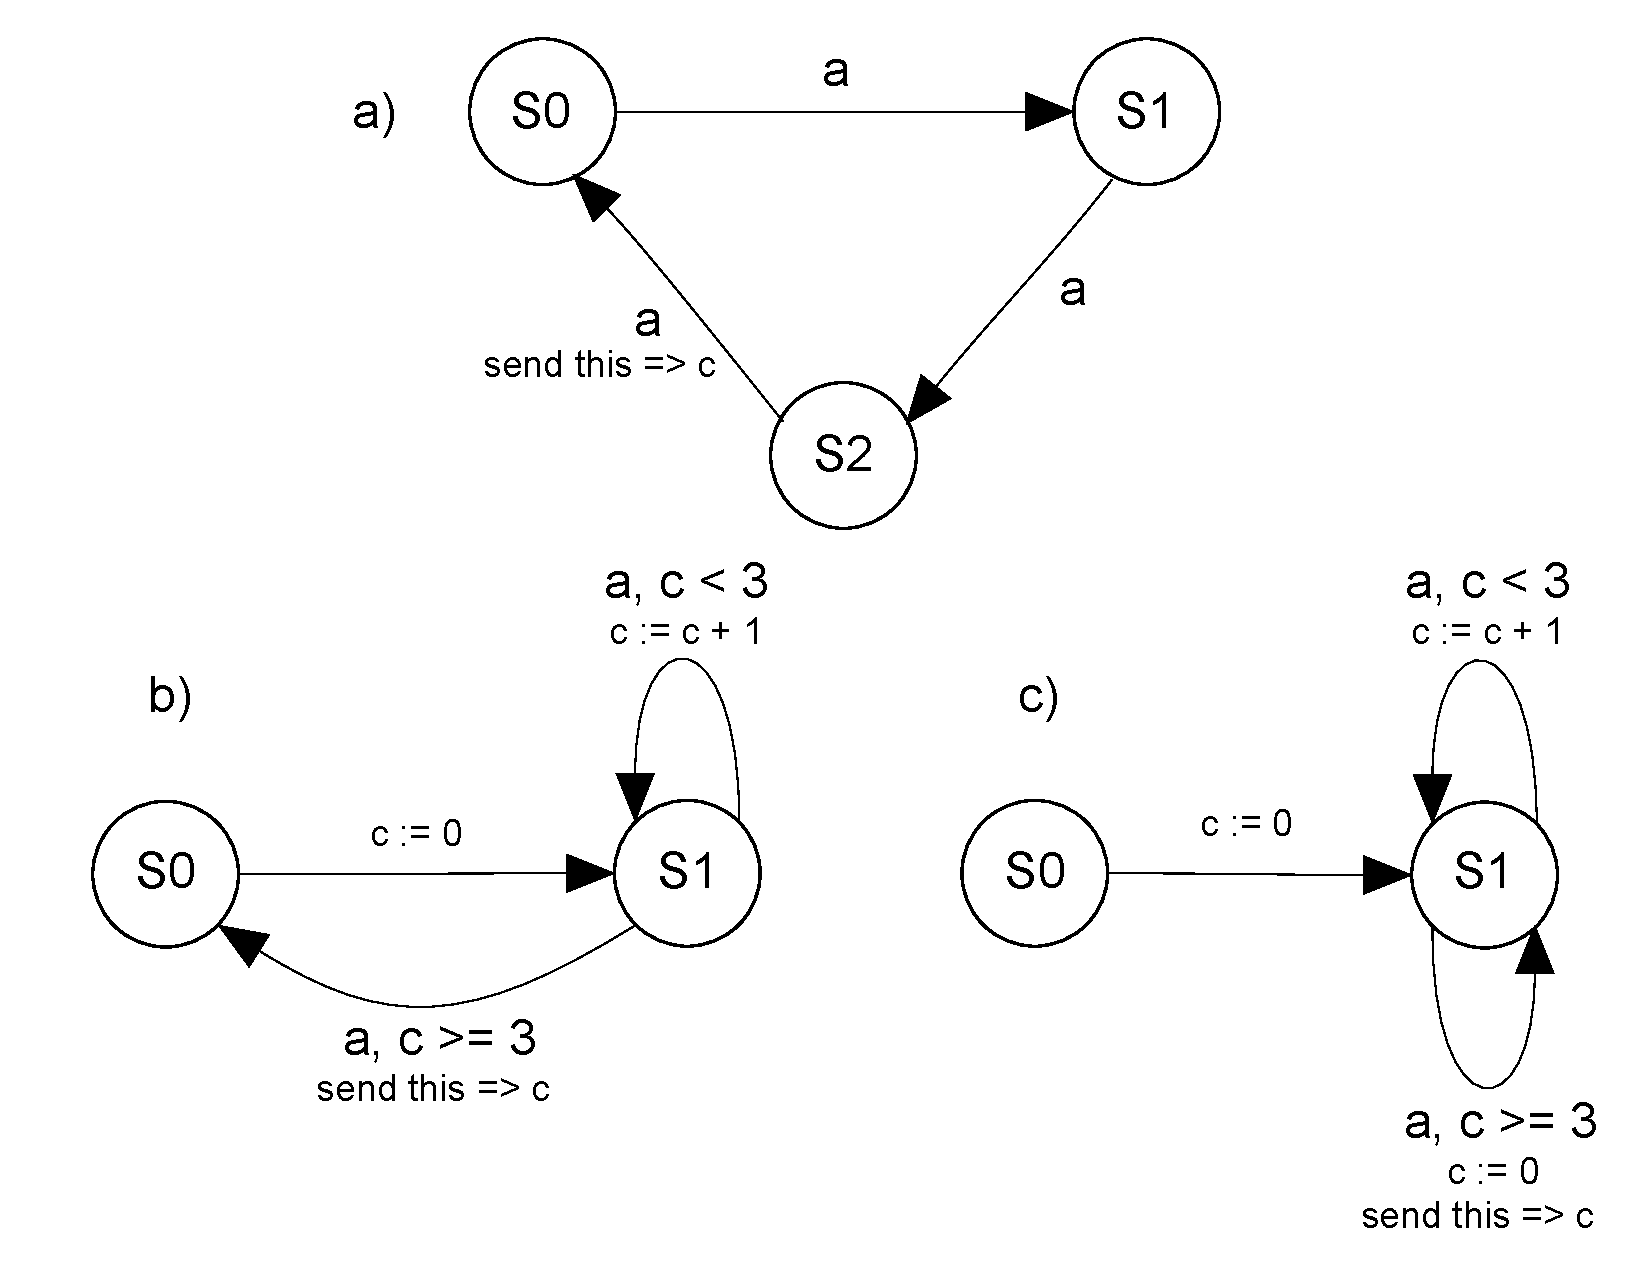
\includegraphics[scale=0.4]{figs/counter.pdf}
  \caption{The transition diagrams of the counter synchroniser.}
  \label{fig:counter}
  \end{figure}


  \item The selection predicate $\rho$

In a given state $k$ for each output channel $\omega_{m}$ we note all $i$ on which $\rho_{ki}^{m}$ is true. Those message values must be stored in a previous state and recalled in state $k$. It is expected that the boolean vector $\omega_{i} = \rho_{ki}^{m}$ has only very few true elements.

Consequently the storage mechanism that \ak\ provides for synchronisers is in the form of individual \emph{store} variables, which are associated with input channel types.

\textbf{Example: the binary zip synchroniser}  Zip2 receives messages on its input channels and sends their concatenation to the output channel. In the resulting concatenation there's exactly one message from each input channel and those messages are ordered as they received.

The zip2 transition diagram is given in Figure \ref{fig:zip2}. The message received in the current transition is referred by a keyword \emph{this}. $ma$ and $mb$ are the store variables associated with the input channels $a$ and $b$ respectively. The statement \emph{send} indicates a sending of a message to an output channel.

  \begin{figure}[here]
  \centering
  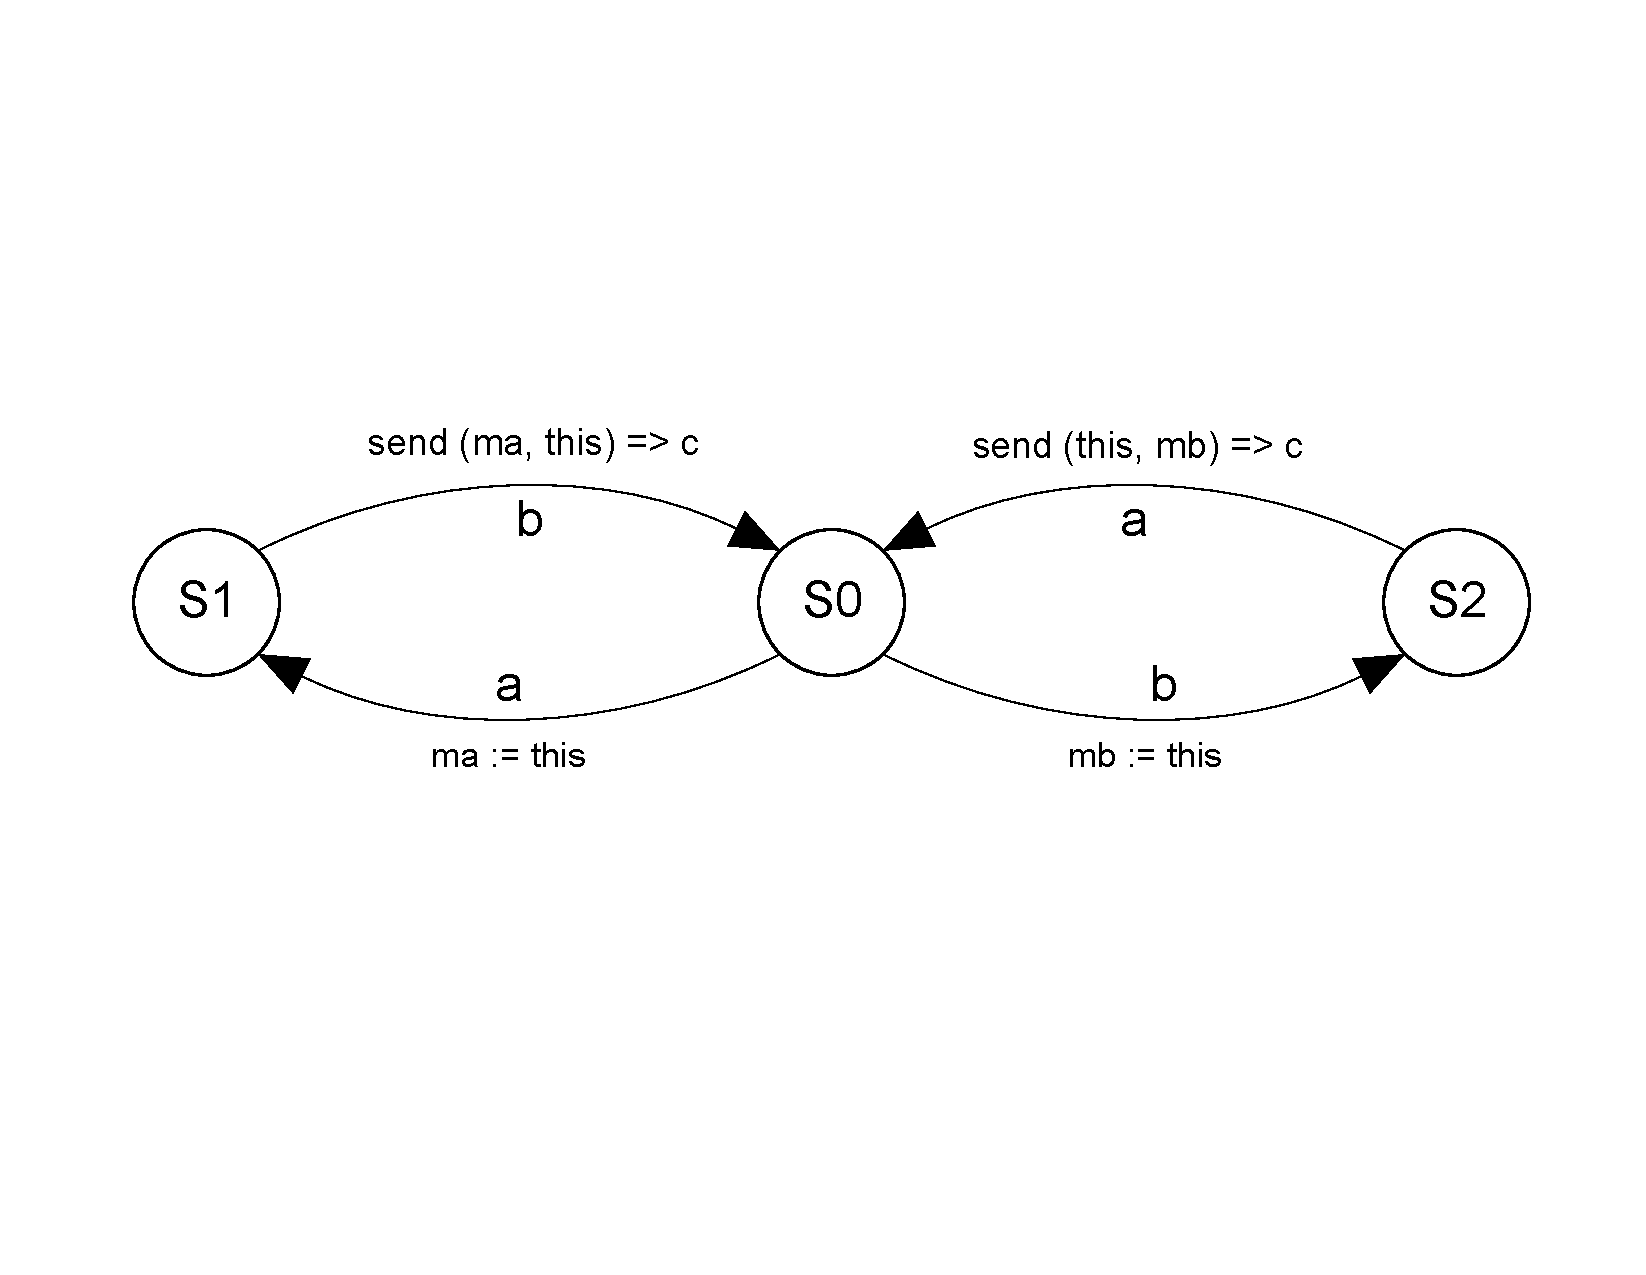
\includegraphics[scale=0.4]{figs/zip2.pdf}
  \caption{The transition diagram of the zip2 synchroniser.}
  \label{fig:zip2}
  \end{figure}

Mathematical model $S_{zip2} = (\Phi, \; \Pi)$, where
  \begin{itemize}
  \item[] $\Phi = (A, \; S, \; T)$,
    \begin{itemize}
    \item[] $C = (a, \; b)$, $P = (true)$, $A = C \times P = ((a, \; true), \: (b, \; true))$,
    \item[] $S = (s_{0}, s_{1}, s_{2})$, $s_{0}$ -- start state,
    \item[] $T$:
      \begin{tabular}{c|c|c|c}
      $A$ \textbackslash $S$ & $s_{0}$ & $s_{1}$ & $s_{2}$\\
      \hline
      $(a, \; true)$ & $s_{1}$ & $s_{1}$ & $s_{0}$\\
      \hline
      $(b, \; true)$ & $s_{2}$ & $s_{0}$ & $s_{2}$\\
      \end{tabular}
    \end{itemize}
  \item[] $\Pi \: : \: S \times \Omega \to V$,
    \begin{itemize}
    \item[] $\Omega = (c)$,
    \item[] $V = ((a, \; b), \: (b, \; a))$
    \end{itemize}
  \end{itemize}

An output message is emitted when a transition happens either from the state $s_{1}$ or the state $s_{2}$. These states are reached in two paths:
  \begin{itemize}
  \item[]
$W_{0} = ((s_{0}, \; a), \: (s_{1}, \; b))$

$\Pi \; (s_{1}, c) = \psi_{\sqcap} \; \{\mu_{0} = a \: | \: \rho_{10}^{c} \; (s_{0}) = 1, \mu_{1} = b \: | \: \rho_{11}^{c} \; (s_{1}) = 1\}$, $k = 1$, $i = 0,1$
  \item[]
$W_{1} = ((s_{0}, \; b), \: (s_{2}, \; a))$

$\Pi \; (s_{2}, c) = \psi_{\sqcap} \; \{\mu_{0} = b \: | \: \rho_{20}^{c} \; (s_{0}) = 1, \mu_{2} = a \: | \: \rho_{22}^{c} \; (s_{2}) = 1\}$, $k = 2$, $i = 0,2$ 
  \end{itemize}
  \end{enumerate}


\section{Synchroniser code}

\begin{figure}[h!]
\begin{framed}
\small
\begin{grammar}
[(colon){$\rightarrow$}]
[(semicolon)$|$]
[(comma){}]
[(period){\\}]
[(quote){\begin{bf}}{\end{bf}}]
[(nonterminal){$\langle$}{$\rangle$}]
<synchroniser>:"synch",<name>,[<confs>],<params>,"\{"<decls>,<trans>"\}".

<confs>:"{\tt [}",<conf>,[",",<conf>]*,"{\tt ]}".
<conf>:<id>

<params>: "(",[<inparam>,[",",<inparam>]*],"{\tt |}",[<outparam>,[",",<outparam>]*],")".

<inparam>:<chan>,[":",<indepth>].
<chan>:<id>.
<indepth>:<var>;<const>.
<var>:<id>.

<outparam>:<chan>,[":",<depth-exp>].
<depth-exp>:<const>;<var>;<var>,"{\tt+}",<shift>;<var>,"{\tt -}",<shift>.
<shift>:<const>;<conf>.

<decls>:[<store-decl>;<state-decl>]*.
<store-decl>:"store",<var>,"{\tt :}",<chan-tail>,[<var>,"{\tt :}",<chan-tail>]*.
<state-decl>:"state",<type>,<var>[",",<var>]*.
<type>:"int(",<const>,")";"enum(",<id>,[",",<id>]*,")".
<chan-tail>: <chan>;<tail>.

<trans>:<tran>[",",<tran>]*.
<tran>:[<label>,":"],[<on-clause>],[<do-clause>],[<send-clause>],[<goto-clause>].

<on-clause>:"on",<chan-cond>;"elseon",<chan-cond>.
<chan-cond>:<primary>["{\tt \&}"<guard-exp>].
<primary>:<chan>,[".",<secondary>].
<secondary>:"{\tt@}",<id>;"{\tt else}";"?",<id>;["?",<id>]<pattern>.
<pattern>:"(",<id>,[",",<id>]*,["{\tt||}",<tail>, ")".
<guard-exp>:<int-exp>.
<tail>:<id>

<do-clause>: "do",<assgn>,[",",<assgn>]*.
<assgn>:<id>,"{\tt :=}",<int-exp>; <id>,"{\tt :=}",<data-exp>.

<send-clause>: "send", <dispatch>,[",",<dispatch>]*.
<dispatch>: <msg-exp>,"{\tt =>}", <chan>.
<msg-exp>: "{\tt @}",<int-exp>; "?",<id>; ["?",<id>],<data-exp>;"nil".
<data-exp>: <primary-mes>; "(",<primary-mes>, ["," <primary-mes>]*,")".
<primary-mes>: <var>;<var>=<int-exp>;"this".
<goto-clause>:"goto",<label>.

\end{grammar}
\end{framed}
\caption{The syntax of the \ak\ synchroniser}
\end{figure}

Explain what every language construct means


\section{Execution order of synchroniser\label{execod}}
Algorithm of the execution of synchronisers, in which order transitions execute


\section{The implementation of the compiler}
The implementation of the compiler frontend in OCaml \cite{realworldocaml}, with code generation to a python structure.

  \subsection{Type checking}
  \subsection{Synchroniser passport}
%  \subsection{Dead code elimination}
%Based on Section \ref{execod}.
